As early as 1964, Goffman~\cite{goffman64OnRelevanceAsAMeasure}, a
mathematical information science pioneer \cite{harmon08RememberingWG},
notes that the relevance of documents in a list has to depend on the
documents preceding it.  More recently, work on
MMR~\cite{carbonell98MMR} was one of the first to formalize
diversification as a mathematical optimization criterion; MMR has
proved one of the most popular diversity approaches.  We note that the
results as derived in the last section formally motivate much of MMR and now
we discuss further connections between optimizing expected $n$-call@$k$ 
and other diversification approaches proposed in the literature.

\subsection{Greedy Submodular Optimization}

%% SHENGBO: This section is almost entirely about Exp-1-call@k not n-call
%%          since all of this text predates SIGIR 2012.  Do any of these
%%          comparisons extend to n-call?  Not all do, but you should
%%          make any connections where possible -- i.e., a max is allowed.  
%%          I modified the last item on rank-based objectives to
%%          mention n-call.

\cite{agrawal09diversifying} proposes a set-based objective function
to answer ambiguous web queries in a setting where there exists a
predefined taxonomy of information, and that both queries and
documents may belong to more than one category according to this
taxonomy. The proposed set-based objective function aims at maximizing
the probability that the average user finds at least one useful
resulting document retrieved within the top $k$
results. Mathematically, this objective function
is defined below:
%% SHENGBO - IA-Select is the greedy algorithm, not the objective 
%
%% SHENGBO - don't define new notation, c is really equivalent to topics
%%           t and you should use notation for S_k, S_k^*, s_i, s_i^* defined previously.
\begin{align}
	P(S_k|\vec{q}) = \sum_{t\in T} P(t|\vec{q}) \left( 1 - \prod_{s_i\in S}(1-V(r_i| \vec{q}, s_i))\right) 
\label{eq:diversifykObjectiveFunction}
\end{align}
where $V(r_i| \vec{q}, s_i)$ broadly defines the
likelihood that a document $s_i$ satisfies the query $\vec{q}$ given the
topics of the query $\vec{q}$ and the document $s_i$, i.e., $t$ and $t_i$, respectively\footnote{We 
have slightly adapted notation in the above equation from the original 
for consistency with our previous definitions in this article.}.
%% SHENGBO - learning has nothing to do with this paper - LDA in the
%%           PLMMR paper was inappropriately applied (it is an admixture model,
%%           not a mixture model) and we have not proposed any learning in
%%           approach in this work -- indeed we suggested non-learning similarity 
%%           metrics could be converted to topic probabilities to match MMR.
%, and note also that the taxonomy of $c$ given the query
%and document is not learnt by some unsupervised model, but
%hand-crafted.
The authors point out that one particular advantage of this set-based objective 
function is that it is submodular, hence permitting a $\left( 1 - \frac{1}{e} \right)$
approximation if optimized greedily as shown in~\cite{Nemhauser:MathProg1978}.
%
Referring back to our results shown in Equation~\ref{eq:partial_simp}~and~\eqref{eq:diversifykObjectiveFunction} from 1-call@$k$, we note that the objective function in Equation \eqref{eq:diversifykObjectiveFunction} is related with ours, but it is unclear if Equation \eqref{eq:diversifykObjectiveFunction} can be derived from the 1-call@$k$ objective, suggesting potential improvements in \cite{agrawal09diversifying}. 
%writing out the mathematical expectation in terms of the sum over all
%possible topics (e.g., taxomony in \cite{agrawal09diversifying}) the
%weighted relevance where weights are the topic distributions below
%%% SHENGBO: the following is not correct, look at Eq (7)
%%%          you need P(t_k=t|s_k) and i={1..k-1}
%%%
%%%          This means P(c|q) should be replaced with P(t|\vec{q}) * P(t_k=t|s_k)
%%%          if deriving from 1-call@k... it's not clear whether *their* result
%%%          can be derived from an objective and model and this suggests their
%%%          approach may be improved.
%\begin{align*}
%    \ExpOneCall(S_k,\vec{q}) & = \mathbb{E} \left[\left. \bigvee_{i=1}^{k}r_i=1 \right| s_{1},\dots, s_{k},\vec{q} \right], \\
%    												 & = \sum_{t\in T} P(t|\vec{q}) \left( 1 - \prod_{i=1}^{k}(1-p(t_i = t| q, s_i))\right) 
%\end{align*}
%Clearly our proposed objective is equivalent to the objective
%Equation~\eqref{eq:diversifykObjectiveFunction} proposed
%in \cite{agrawal09diversifying} when one replaces the likelihood
%function $V(s|\vec{q}, c)$ by $p(t_i = t| \vec{q}, s_i)$. 
More recently, \cite{Vargas:SIGIR2012} introduce several interesting formal probabilistic
relevance models to instantiate $V(r_i| \vec{q}, s_i)$, which are more
appopriate in modeling the relevance in a probabilistic
framework. Furthermore, \cite{Vallet:SIGIR2012} propose to introduce a
user as an explicit random variable in state of the art
diversification methods, thus developing a generalized framework for
personalized diversification.

Another recent interesting instantiation of $V(r_i|\vec{q},s_i)$ is proposed
in \cite{Zuccon:ECIR2012} motivated by the facilitation location
problem~\cite{Gonzalez:Handbook2007} taken from Operations Research:
for a set of customer ``locations" $D$, one aims at choosing a subset
$S_k$ in $D$ to open $k$ ``facilities" that optimize a graph-theoretic
objective that depends on the cost of opening a facility at each
location and also the distance between each pair of locations. However
all of the described methods do not derive their objective
functions from the expected 1-call@$k$ objective as we have achieved.

\subsection{Portfolio Theory}
\cite{wang09PortfolioTheory} motivates
diversification in set-based information retrieval by a
risk-minimizing portfolio selection approach. Viewing a result set as
an investment portfolio with the objective to maximize return while
minimizing risk, the derived result of~\cite{wang09PortfolioTheory}
mimics both MMR and Exp-$1$-call@$k$ in that the similarity term may
be viewed as \emph{expected portfolio payoff} (relevance) and the
diversity term may be viewed as \emph{expected portfolio risk}, which
increases as the correlations between documents in the result set
increase. 
%% SHENGBO -- you used to have math here for Wang09 which you've omitted.
%%            It's not very clear to say a sum here if you never show it!
%%            (There was not room in CIKM to display this.)
%%
%%            Also I suggest dropping the mention of Shi -- it is not
%%            clear and it interrupts the flow of discussion about wang
%%            and the lead-in to the next section.
%Note that diversification based on portfolio theory is
%extended in \cite{Shi:SIGIR2012} by introducing latent factors for
%collaborative filtering tasks. 

One major difference in the
framework~\cite{wang09PortfolioTheory} is that rather than computing
the diversity term via a max (MMR) or product (Exp-$1$-call@$k$) the
portfolio theory derivation uses a summation: 
\begin{align}
s_{k}^{*} = \argmax_{s_{k}} \left[ \Sim^{\text{BM25}}(s_k,\vec{q}) \hspace{-.7mm} - \hspace{-.7mm} \lambda \sum_{i=1}^{k-1} \omega_{i} \Sim^{\text{TFIDF}}(s_i,s_k) \right]
\end{align}
Here, $\lambda$ is a manually tuned weight parameter, $\omega_1,\ldots,\omega_k$
are the weights of each position in the result set (for lack of more informed
choice, we chose a uniform weighting),
$\Sim^{\text{BM25}}(s_k,\vec{q})$ is the BM25~\citep{bm25} probabilistic
relevance score of document $s_k$ w.r.t.\ query $\vec{q}$ and
$\Sim^{\text{TFIDF}}(s_i,s_k)$ is a TFIDF~\citep{salton83Introduction}
similarity metric between two documents $s_i$ and $s_k$ represented as term
frequency vectors.


We examine the implications of this next.

\subsection{Set Covering}
Yue and Joachims~\cite{yue081224Predicting} propose a set covering
approach for training SVMs to predict diverse result sets for
information retrieval.  In their work, they equate subtopics with
words and build a loss function for SVM training that penalizes result
sets according to the sum of weights of query-relevant words
\emph{not} covered by the result set.  While their approach provides a
``hard'' set-covering view of diversity, we note that an expansion of
$\tilde{P}(t | S_{k-1}^*)$ used in the diversity term
of~\eqref{eq:1call} provides a ``soft'' latent set-covering
interpretation; that is, $s_k$ is chosen so as to best cover (in a
probabilistic sense) the latent topic space not already covered by $\{
s_1^*,\ldots,s_{k-1}^* \}$.  Formally, expanding the product in
$\tilde{P}(t | S_{k-1}^*) = \prod_{i=1}^{k-1} \left(1 -
P(t_{i}=t|s_{i}^{*})\right)$, collecting terms and writing it as a
series, we arrive at a form that reflects the inclusion-exclusion
principle applied to the calculation of probability that topic $t$ is
covered by $\{ s_1^*,\ldots,s_{k-1}^* \}$:
\begin{align}
& \prod_{i=1}^{k-1} \left(1 - P(t_{i}=t|s_{i}^{*})\right) \nonumber \\
& = 1 - \left[ \sum_{i=1}^{k-1} P(t_{i}= t|s_{i}^{*}) - \sum_{i=1}^{k-1}\sum_{j=1}^{k-1}P(t_{i}= t|s_{i}^{*})P(t_{j}= t|s_{j}^{*}) + \dots - (-1)^{k-1}\prod_{i=1}^{k-1}P(t_{i}=t|s_{i}^{*})\right] \label{eq:setcover}
\end{align}

This result has a natural interpretation: the first summation term
determines the coverage of topic $t$ by each document $s_i$ ($1 \leq i
\leq k-1$) currently in the result set, the second double summation
term corrects the first term by removing the joint probability mass
from all pairs of documents that was double counted, and so on
according to the principle of inclusion-exclusion.
\eqref{eq:setcover} not only provides a probabilistic set covering
view of Exp-$1$-call@$k$, but it also suggests that a portfolio
approach to diversity using only the first summation would overcount
each document's contribution to the diversity metric according to this
set covering perspective.

The inclusion-exclusion principle calculation provided by the second
term in Equation~\ref{eq:setcover} is illustrated
in~Figure~\ref{fig:inclusionExclusionPrinciple}. In words, this term
is calculating the total topic probability coverage of $t$ by all
selected items $\{ s_1^*,\ldots,s_{k-1}^* \}$ by properly applying the
inclusion-exclusion principle to ensure that overlapping probability
coverage is not double counted. Then referring back to
Equation~\ref{eq:partial_simp}, we note that $s_k$ is chosen by
maximizing a weighted sum over topics, where each topic weight is
determined by its relevance to the query $\vec{q}$, the item $s_k$,
and penalized (i.e., due to the $1 - $) by the topic coverage of $t$
by the set $\{ s_1^*,\ldots,s_{k-1}^* \}$ to naturally encourage
diversity.  We note that this is a soft probabilistic version of the
``in or out'' topic coverage approach of WSL.
%% SHENGBO: WSL is not defined!!!

%%%%%%%%%%%%%%%%%%%%%%%%%%%%%%%%%%%%%%%%%%%%%%%%%%%%%%%%%%%%%%
\begin{figure}[t!]
\begin{center}
\centerline{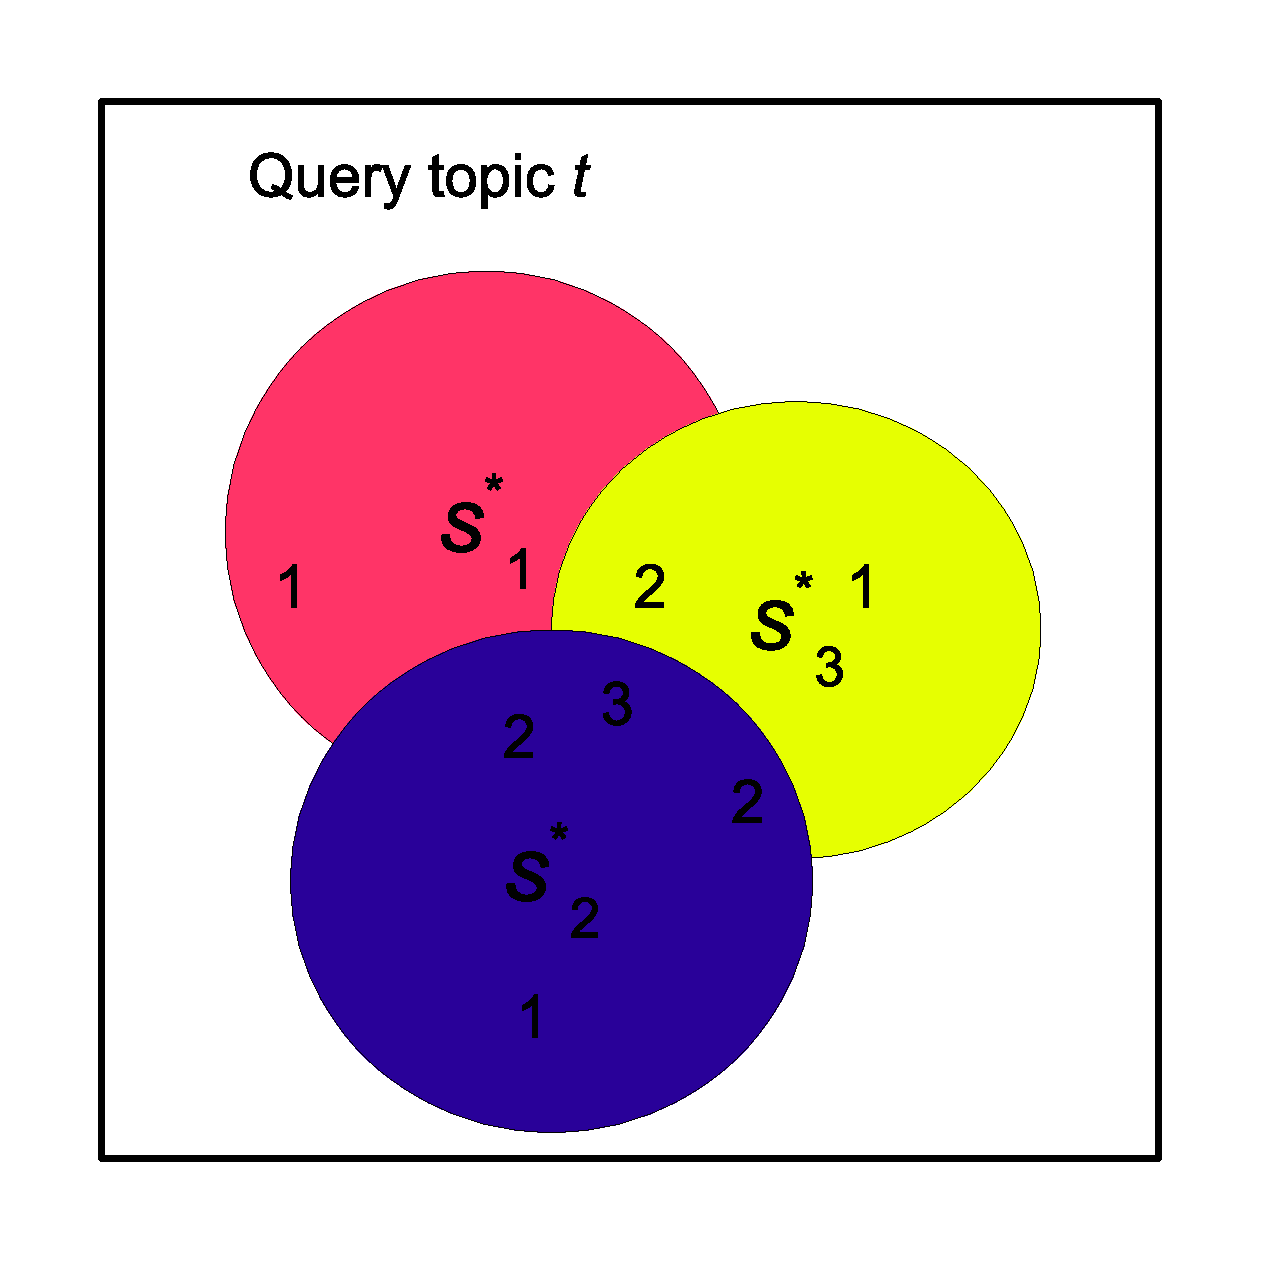
\includegraphics[scale = 0.4]{inclusionExclusionPrinciple}}
\caption[Inclusion-exclusion principle.]{Inclusion-exclusion principle. The sets represent candidate
items $s$ for a query, and the area covered by each set is the
``information" covered by that item for query topic $t$. Numbers on different areas
indicates the number of sets that share these areas. }
\label{fig:inclusionExclusionPrinciple}
\end{center}
\end{figure}
%%%%%%%%%%%%%%%%%%%%%%%%%%%%%%%%%%%%%%%%%%%%%%%%%%%%%%%%%%%%%%

\subsection{Subtopic Relevance Models} 

We use a subtopic relevance model that is a simplified version of the
model in~\cite{plmmr} with fewer dependence assumptions.  In other
work, Zhai {\it et al}~\cite{zhai03Beyond} present an empirical risk
minimization view of dependent document retrieval from a subtopic
perspective, where they derive a formalization of the
\emph{greedy} selection step that is similar to MMR and to a lesser
extent, Exp-$1$-call@$k$.

\subsection{Set-based Relevance Objectives} 

Chen and Karger~\cite{chen06Less}, whose derivation we extended,
directly optimize $1$-call@$k$, but their intention is not to
formalize MMR and instead use na\"{i}ve Bayes to directly evaluate
\eqref{eq.ncall}.  Agrawal et al~\cite{agrawal09diversifying}
and Santos et al (xQuad)~\cite{santos2010xquad} both specify set-based
diversity metrics \emph{very} similar to Exp-$1$-call@$k$ but do not provide
formal derivations as we have done in this work. 

\subsection{Ranking Based Objectives} 

Finally, returning to our introductory motivation, Wang and
Zhu~\cite{wangzhu10} have shown that natural forms of result set
diversification arise via the optimization of average
precision~\cite{ap} and reciprocal rank~\cite{mrr}.  Both of these
methods share the view of directly optimizing a
\emph{ranking-based} objective, whereas this paper proposes a novel
derivation from the alternate view of optimizing a \emph{set-based}
objective w.r.t.\ a subtopic model of relevance.  However, even though
Exp-$n$-call@$k$ is a set-based objective, an indirect consequence of
(and motivation for) greedily optimizing it is that documents added
earlier yield a greater increase in objective than those added later;
this yields a natural rank ordering on the greedy Exp-$n$-call@$k$
result set.

%% SHENGBO: I removed the table because you are referring to learning and
%%          a lot of traits that were relevant to PLMMR in SIGIR 2010 that
%%          are no longer relevant now.  Either you need to do an entirely
%%          new analysis relevant to this paper and its objectives, or just
%%          drop it as I did.
%%
%%          Old content is checked in under related_work_unused.tex

